\section{Design of the Controller}\label{designController}
The design of the controller is based on the root locus plot, where the final location of the poles in closed loop can be seen.

The root locus of the system with a proportional controller can be seen in \figref{rlocusCubli2}.

\begin{figure}[H]
	\centering 
	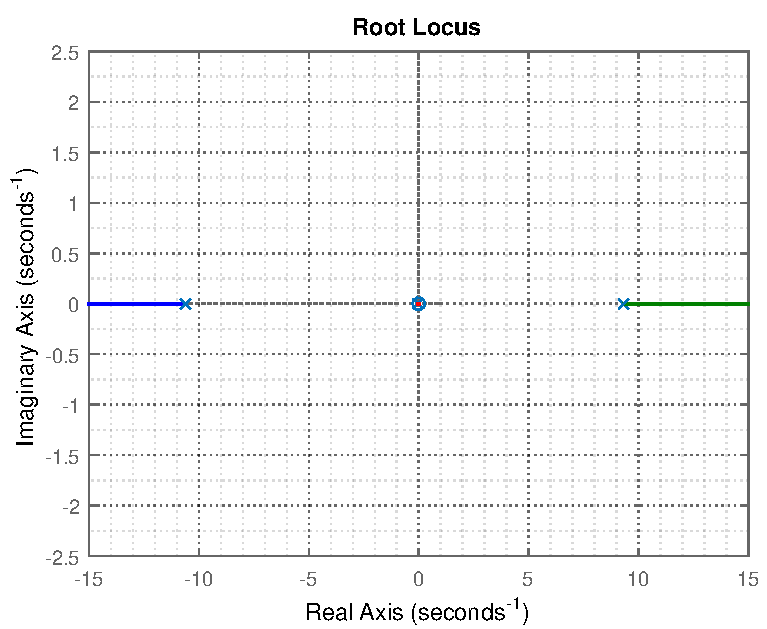
\includegraphics[scale=.75]{figures/rlocusCubli}
	\captionof{figure}{Root Locus of the system. It has  one zero \si{(s=0)}, and three poles \si{(s=-10,5014}, \si{s=-0,0283} and \si{s=9,3531}).}
	\label{rlocusCubli2}
\end{figure}

Looking at the root locus it can be derived that the system can not be controlled using only a proportional controller because there is always a pole in the RHP no matter the gain.

However, a first approximation of the system's behavior in closed loop can be done through a proportional controller. Such a system is tested with a gain of 10 as a controller. The final closed loop poles are placed at \si{-40,4198;\ -0,0018\ and\ 39,2448}. In \figref{closedLoopResponse} it is shown the response of the simulation and the one from the real setup with this proportional controller.

\begin{figure}[H] 
	\centering 
	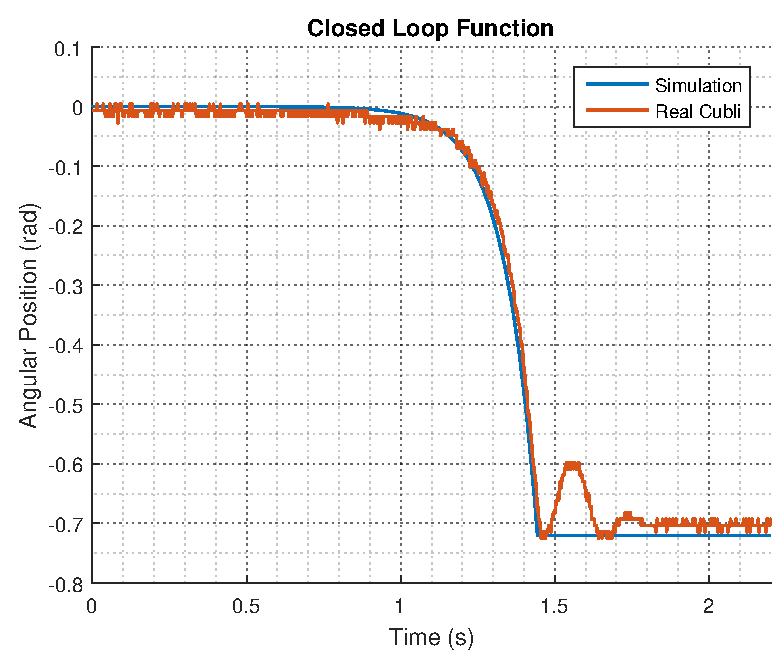
\includegraphics[scale=0.75]{figures/closedLoopResponse}	
	\caption{Behavior of the closed loop function with a proportional controller, both in simulation and reality.}
	\label{closedLoopResponse}
\end{figure}
%
It is clear that, upon application of a \SI{0}{rad} reference and a minimal initial offset, the closed loop function with only a gain of 10 has an unstable response. Then the branches of the root locus need to be changed by means of the addition of poles and zeros in the controller.

As there exists one pole in the Right Half Plane (RHP), the controller must also have one there to create two branches which can be attracted to the Left Half Plane (LHP).

Then, two zeros must be placed in the LHP to make the branches enter in the stable region of the plot.

It is also important for the number of poles to be greater than the number of zeros so that the controller is feasible in reality. This means that two poles need to be placed somewhere so they don't affect the behavior of the final system. This can be achieved if they are placed in the LHP and far from the imaginary axis.

Finally, the gain must be adjusted to make the closed loop poles to be in a stable location. The resultant Root Locus can be seen in \figref{RLControllerZoom}.

\begin{figure}[H]
	\centering 
	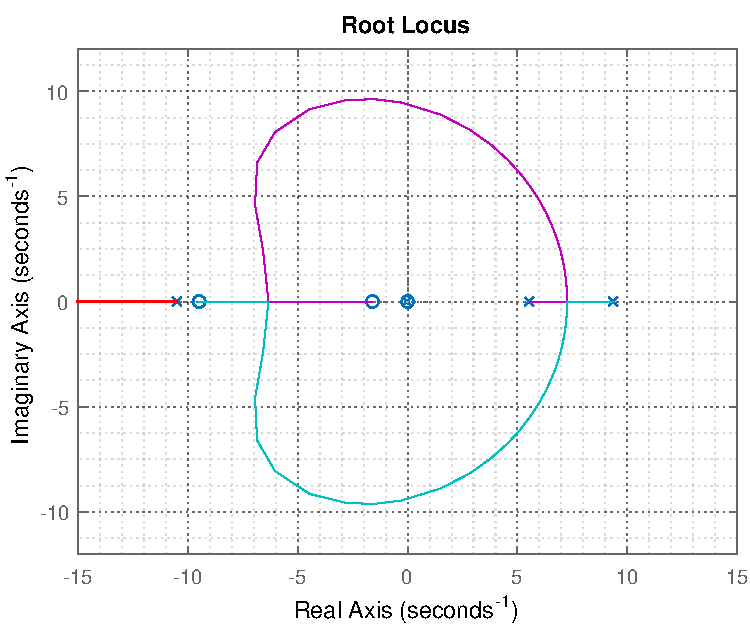
\includegraphics[scale=.65]{figures/RLControllerZoom}
	\captionof{figure}{Root Locus of the final system.}
	\label{RLControllerZoom}
\end{figure}
%
The final system looks like \figref{blockDiagramController} and the transfer function of the controller is give by \eqref{ControllerLaplace}.
%
\begin{figure}[H]
	\begin{tikzpicture}[ auto,
thick,                         %<--setting line style
node distance=1.5cm,             %<--setting default node distance
scale=0.75,                     %<--|these two scale the whole thing
every node/.style={scale=0.62}, %<  |(always change both)
>=triangle 45 ]

%-- Blocks creation --%
\draw
% DIRECT TERM %
node[shape=coordinate][](input1) at (0,0){}
node[shape=coordinate][](feed) at (0.5,0){}
node(sum1) at (2,0) [sum] {$\sum$}
node(controller) at (4,0) [block]{\Large $D(s)$}
node(plant) at (6,0) [block]{\Large $G(s)$}
node[shape=coordinate][](DummyNode) at (5,-1.5){}
node[shape=coordinate][](FeedbackNode) at (7.5,0){}
;

%-- Block linking --%
% INPUT %
\draw[-](input1)        -- node{\Large $U(s)$}(feed);
\draw[->](feed)  -- (sum1);

% OUTPUT %
\draw[-](plant)  -- (FeedbackNode);
\draw[->](FeedbackNode)       -- node {\Large $Y(s)$} (9,0);

% DIRECT TERM %
\draw[->] (sum1)            -- (controller);
\draw[->] (controller)       -- (plant);

% FEEDBACKS %
\draw[-] (FeedbackNode)  |- (DummyNode);
\draw[->] (DummyNode)  -| (sum1);

%-- Nodes --%
\draw%--------------------------------------------------------------
node at (input1)            [shift={(-0.04, -0.05 )}] {\Large \textopenbullet}
node at (FeedbackNode)      [shift={(0, -0.07 )}] {\Large \textbullet}
;
%-- Summation signs --%
\draw%--------------------------------------------------------------
node at (sum1) [right = -6.6mm, below = .6mm] {$+$}
node at (sum1) [right = -3mm, below = 3.9mm]  {$-$}
;

\end{tikzpicture} 
	\centering
	\caption{Block diagram of the final controlled system.}
	\label{blockDiagramController}
\end{figure}
%
Where
%
\begin{flalign}
	\eqOne{D(s)} {0,62737 \cdot \frac{(0,1054\ s + 1)\cdot (0,6254\ s + 1)}{(0,1805\ s - 1) \cdot (0,01\ s + 1) \cdot (0,005\ s + 1)} =} \eqTwo{= -4582,2 \cdot \frac{(s + 9,488)\cdot (s + 1,599)}{(s - 5,54) \cdot (s + 100) \cdot (s + 200)}} 
	\label{ControllerLaplace}
\end{flalign}
%
The stability of the controlled system can be then analyzed using the Nyquist plot of the controller and the plant together in open loop, as seen in \figref{nyquistController}.

\begin{figure}[H] 
	\centering 
	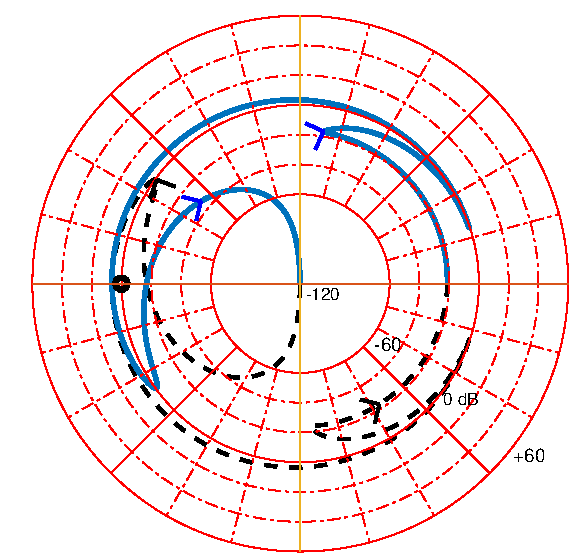
\includegraphics[scale=0.55]{figures/nyquistController}	
	\caption{Nyquist plot of the system with the controller.}
\end{figure}	\label{nyquistController}

Now there are two poles in the RHP and the number of encirclements around -1 equals -2 (they are counterclockwise). 
This means that the system should be stable (see \secref{sec:stabilityAnalysis}), as the number of zeros in the RHP becomes 0.
